\chapter[Produto]{Produto}


 Diagrama de fluxo de sinais geral do Robarco pode ser observado na figura \ref{fg1}.
 
 \begin{figure} [!htp]
 	\centering
 	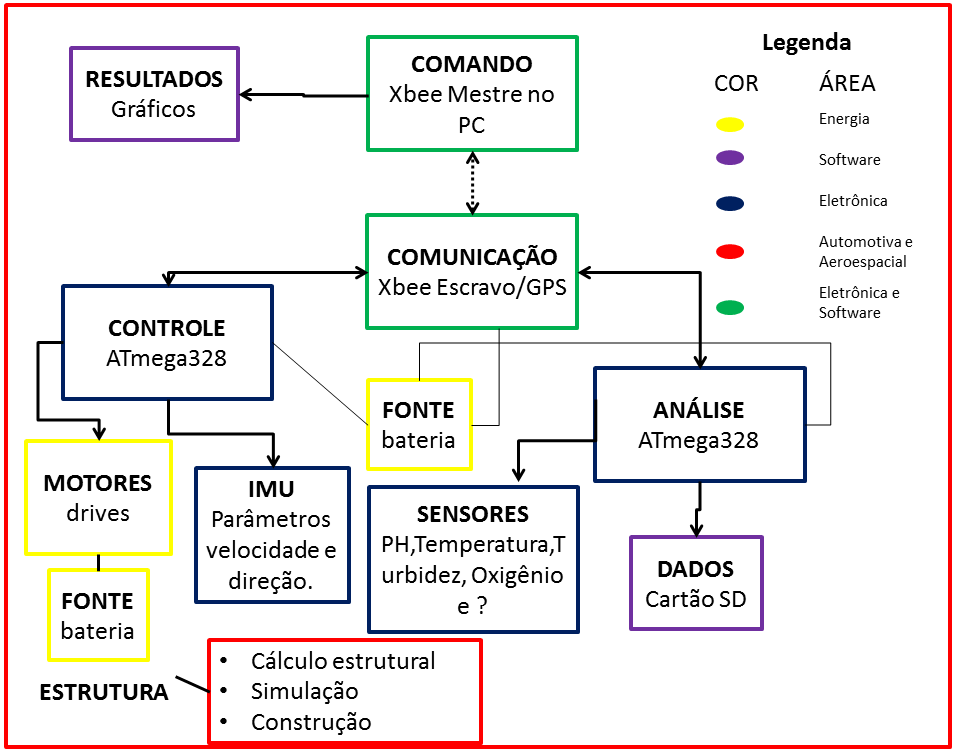
\includegraphics[scale=0.7]{figuras/diagramaGERAL}
 	\caption{Diagrama de fluxo de sinais geral. Demonstra o funcionamento geral e como os componentes serão conectados. Assim podemos desmembrar o problema em tarefas mais simples.}
 	\label{fg1}
 \end{figure}
% %\FloatBarrier

\section{Subgrupo Comunicação}
Xbee

Para controlar e receber os dados a distância escolhemos a tecnologia da Xbee Fig. \ref{Xbee} por sua compatibilidade com \textit{standalone} personalizado "Robarcoino" (nossa versão do Arduino) e alcance de até 1,5 km de distância em área externa. Usaremos uma mestre conectada a um computador e uma escrava dentro do Robarco.
 \begin{figure} [!htp]
	\centering
	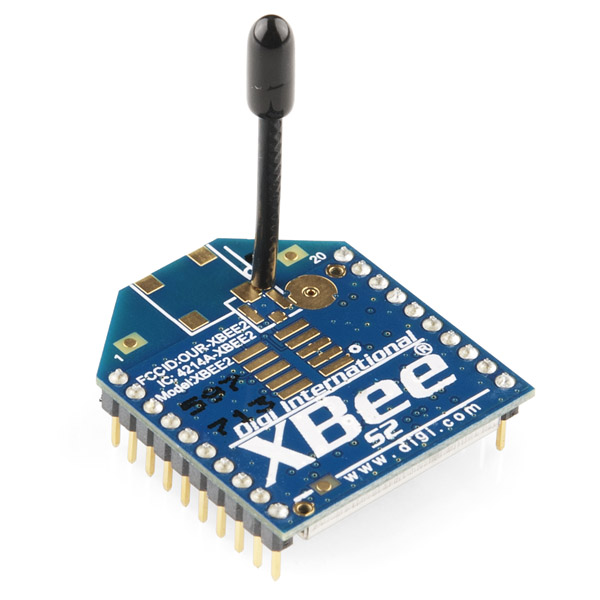
\includegraphics[scale=0.5]{figuras/Xbee}
	\caption{Modulo Xbee pro serie 2 com antena.}
	\label{Xbee}
\end{figure}
%\FloatBarrier
Este módulo XBee PRO da Série 2 é um formato físico de uma família de modems de RF fabricado pela Digi International (MaxStream®) que utiliza o padrão ZigBee IEEE 802.15.4. A Série 2 possui uma melhora no que diz respeito a potência de saída e protocolo de dados, permitindo uma comunicação de forma simples entre microcontroladores, computadores, sistemas, ou qualquer periférico que utilize porta serial.



A ZigBee Alliane junto ao IEEE (Institute of Electrical and Eletronics Engineers) trabalham em conjunto para proporcionar e desenvolver tecnologias para criar um padrão de baixo consumo de energia, baixo custo, segurança, confiabilidade, e com funcionamento em rede sem fios (wireless) baseado em uma norma aberta e global.



Os módulos RF padrão ZigBee operam na freqüência ISM (Industrial, Scientific and Medical), sendo na Europa de 868 MHz (1 canal), 915 MHz (10 canais) nos Estados Unidos e 2,4 GHz (16 canais) em outras partes do mundo, e não requerem licença para funcionamento. Eles foram criados para economizar o máximo de energia e se comunicarem uns com os outros na forma e roteamento de sinais de forma similar as abelhas que voam aparentemente em Zig-Zag, daí o nome ZigBee, e dessa forma, durante um vôo a trabalho as abelhas em busca de néctar trocam informações com outros membros da colmeia sobre distância, direção e localização de onde encontrar pólen. Este modo de configuração de rede permite a dispositivos com ZigBee encontrarem outros dispositivos de forma apropriada, automática e configurar vários caminhos possíveis entre cada nó da rede para a passagem da informação, pois já que numa única rede podem existir mais de 65 mil nós ZibBee então a rede pode ser distribuída por centenas ou milhares de quilômetros quadrados sem prejuízo de comunicação. E se algum nó falhar, uma rota alternativa é automaticamente encontrada, simplesmente mudando o percurso da informação.



As Redes ZigBee oferecem uma excelente imunidade contra interferências, sendo ideal para aplicações industriais, mesmo em ambiente hostil e de fortes ruídos, pois mantem a integridade da comunicação. Também pode ser destinado ao uso residencial, pois possui longo alcance e baixíssimo consumo.


Características:
Performance
- Rendimento da Potência de saída: 63 mW (+18 dBm) / 10 mW (+10 dBm) EIRP;
- Alcance em ambientes internos/zonas urbanas: 90m;
- Alcance de RF em linha visível para ambientes externos: 1,5Km;
- Sensibilidade do receptor: -102 dBm (1\% PER);
- Freqüência de operação: 2,4 GHz;
- Taxa de dados de RF: 250 Kbps;
- Taxa de dados serial (Data Rate): 1.200 bps a 1Mbps;
Alimentação
- Tensão de alimentação: 2,7 à 3,6V;
- Corrente de transmissão (típico): 205 mA em 3,3 V;
- Corrente de Recepção (típico): 47 mA em 3,3 V;
- Corrente de Repouso: 3,5 microA em 25ºC;
Propriedades físicas
- Dimensões: (2,438cm x 3,294cm);
- Peso: 3,5g;
- Temperatura de operação: -40 a +85ºC (industrial);
- Antena integrada no módulo do tipo: Arame (wire whip);
Rede
- Tipo de espalhamento espectral: DSSS (Direct Sequence Spread Spectrum);
- Manipulação de erro: Retransmite novamente (Retries) e reconhecimento (acknowledgements);
- Topologia de Rede: Peer-to-peer (Par-a-par), ponto-a-ponto, ponto-a-multiponto e malha;
- Endereçamento: 65.000 endereços de rede disponíveis para cada canal;
- Opções de filtros: PAN ID, canais e endereços;
- Criptografia: 128-bit AES;
- Número de canais selecionáveis via software: 14 canais de seqüência direta;
Geral
- Faixa de freqüência: 2,4000 - 2,4835 GHz;
- 06 pinos de entrada com ADC 10-bit;
- 08 pinos de entrada/saídas.

Iremos estudar o funcionamento da Xbee através de cinco aula de um professor americano disponibilizadas no Youtube. XBee Basics - Lesson 1 até 5. Usando o guia da figura \ref{xbeeguide}

 \begin{figure} [!htp]
	\centering
	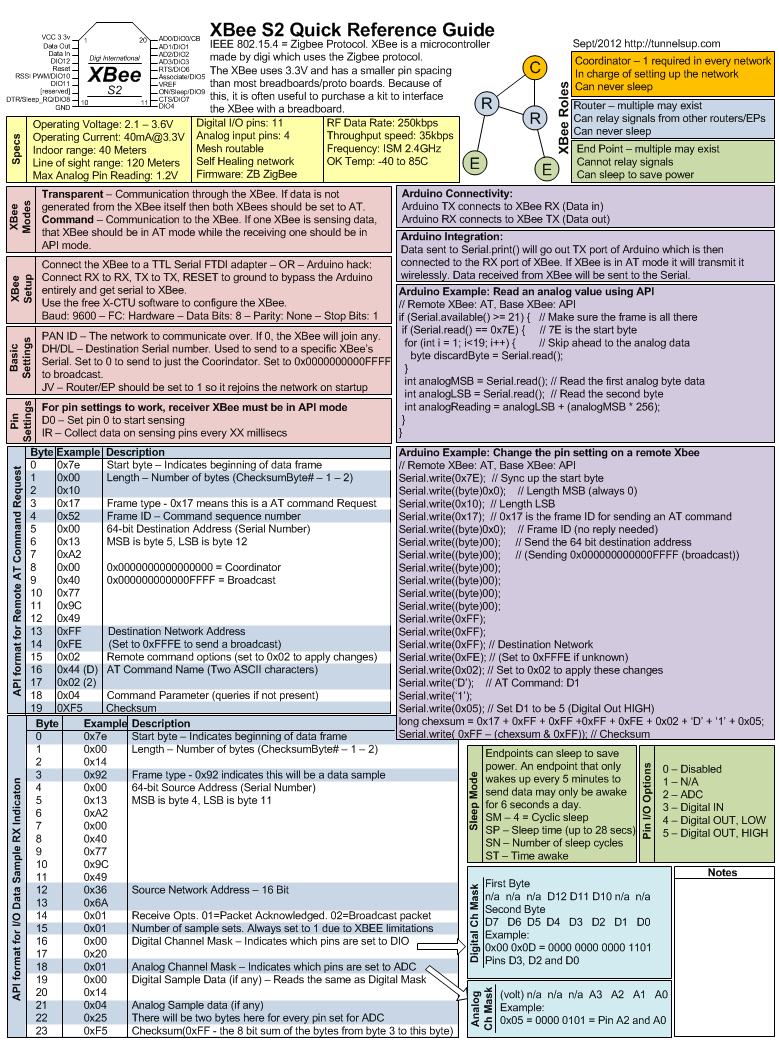
\includegraphics[scale=0.6]{figuras/xbeeguide}
	\caption{Guia de estudos para trabalhar com Xbee. Um resumo com todas as informações relevantes.}
	\label{xbeeguide}
\end{figure}
%%\FloatBarrier



\section{Subgrupo Controle de motores}

IMU

A Unidade de Medida Inercial (IMU) é um dispositivo eletrônico que mede e relata a força específica do corpo, velocidade angular e o campo magnético em torno do corpo, usando uma combinação de giroscópios acelerômetros e barômetros.Um IMU permite que um receptor GPS para trabalhar quando de GPS sinais não estão disponíveis, como em túneis, no interior de edifícios, ou quando a interferência eletrônica está presente.

 \begin{figure} [!htp]
	\centering
	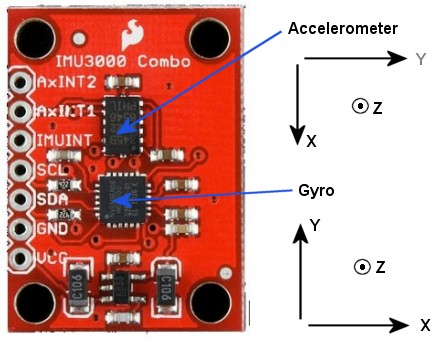
\includegraphics[scale=0.6]{figuras/IMU}
	\caption{Módulo de uma unidade lógica inercial compatível com arduino.}
	\label{IMU}
\end{figure}
%%\FloatBarrier

Motor 


Para obtenção das características necessárias para a escolha do motor, será necessária que haja a estimativa de alguns valores, a fim de se obter informações suficientes para poder realizar posteres cálculos.



Estimativa:O cálculo da potência de eixo do motor depende da resistência ao avanço que o barco possui. A resistência ao avanço é uma função dependende do numéro de Reynolds e do número de Froude. Para tal, a seguir é calculado tais números adimensionais.
\begin{equation}\label{Reynolds}
Reynolds = \frac{V * Lf}{v} 
\end{equation}
Substituindo V por 1,38 m/s, Lf por 1,10 m e v por 0,000001007 $m^2$/s; encontramos 1,507 * $10^6$ .

 
Como o numero de Reynolds é maior que 2100, logo temos escoamento turbulento
\begin{equation}\label{Froude}
	Froude = \frac{V}{\sqrt{g * Lf} }
\end{equation}

Substituindo V por 1,38 m/s, g por 9,81 m/$s^2$ e Lf por  1,10 m; encontramos 0,420.

O número de Froude é menor que 1, logo temos escoamento fluvial
Sendo, 
Lf = Comprimento de linha de flutuação
V = velocidade de avanço do barco
v = viscosidade cinemática da água à 20ºC
g = gravidade
 
Equações dos coeficientes relacionados a propulsão

Velocidade de avanço:Cb é o coeficiente adimensional de finura total. Dado por, segundo o método de Van Lameren:

Cb = 1,37 - (2,02 * V) Lf= 1,37 - (2,02 * 1,38) 1,10 = 1,3516
Sendo, 
Lf = Comprimento de linha de flutuação
V = Velocidade de avanço do barco

é o coeficiente de esteira. Dado por, segundo o método de Taylor:

= -0,05 + 0,50 

=V x VaV 

Sendo, 
= Coeficiente de esteira
V = velocidade de avanço do barco
Va = velocidade com a qual a agua flui para o propulsor



Coeficiente de Declaração do Impulso (t)

t = K * w                       em que: k = 0.50 ~ 0.70 c/ lemes hidrodinâmicos
k = 0.70 ~ 0.90 c/ lemes de chapa dupla e cadaste 
k = 0.90 ~ 1.05 c/ lemes de chapa simples

Método de Schronherr \ref{Schronherr}. 

\begin{equation} \label{Schronherr}
	Pe=Rt*Vs
\end{equation}
 

Onde,
Pe é e a potência efetiva, 
Rt a resistência total 
Vs a velocidade de serviço.

A resistência total é dada pela equação \ref{Rt}. 

\begin{equation} \label{Rt}
   Rt=Rw+Rv+Rb+Ra 
\end{equation}
 

Onde, 
Rw= resistência da onda, desconsiderada no presente trabalho;
Rv= Resistência de viscosidade, dada pela equação 3;
Rb= resistencia do bulbo, desconsiderada no presente trabalho;
Ra= resistência de arrasto, dada pela equação ??

\begin{equation} \label{Rv}
   Rv = 0,5pv^2 * Cf(1+k)*Stotal
\end{equation}
 

Onde, 
p = massa especifica da água;
v= velocidade de serviço;
Cf= Coeficiente de placa plana, dado pela equação 5
(1+K)= Coeficiente de forma, dado pela equação 6
Stotal= Área total estimada.
\begin{equation}
	Cf=\frac{0,075}{(log Re-2)^2}
\end{equation}
               

Onde Re é o numero de Reynolds, que para agua tem valor de aproximadamente 1,006X10-6 , logo Cf= 1,17X10-3.
\begin{equation}
	1+k=1+k1+[(1+k2)-(1-k1)]SappStotal 
\end{equation}
 

Onde, 

1+k1=0,93+(TL)0,2283(BLr)0,92497(0,95-Cp)-521448(1-Cp+0,0225)0,6906

E 
1+k2= valor Tabelado

Ra=0,5v2Stotal.Ca

Onde, 

Cp é dado pela razão entre o  volume do casco e a área transversal vezes o comprimento L,

Cp = vA*L


Com esses valores podemos calcular a potência elétrica, para finalmente calcularmos a potência instalada, dada por

Pi=Pe.margem do mard.t.margem do motor, onde


Margem do mar= valor estimado de 15\%
d= Eficiencia propulsiva estimada de 70\%
t= Eficiência de transmissão estimada de 85\% ( estimando perda das pas e dos eixos de 15\%) 
Margem do Motor= Valor estimado de 10\%


\section{Subgrupo Dados Sensores}

Modulo SD 


Os dados da análise de qualidade da água que forem coletados através dos sensores deverão ser armazenados no Robarco, desta maneira se fez necessário um módulo SD que permita a utilização de um cartão de memória que receberá os dados que forem coletados pelos sensores, assim esses dados servirão de insumos para a elaboração dos gráficos relativos aos parâmetros da água. A vantagem é que caso haja perda de dados na transmissão sem fio poderemos recuperar os dados pela memória do cartão.

O Atmega 328 só possui 32kb de memória e pelo baixo custo de compra e implementação do cartão de memória a equipe optou por essa ação.

Este módulo permite a leitura e escrita em cartão SD (cartão de memória), com fácil ligação ao Arduino e outros microcontroladores. Todos os pinos de ligação estão identificados no módulo, que suporta formatos de arquivo FAT16 e FAT32, e alimentação de 3.3V ou 5V.

A comunicação é feita pela interface SPI (pinos MOSI, SCK, MISO e CS), e o nível de sinal é de 3.3V, exigindo um divisor de tensão para ligação à microcontroladores que trabalhem com 5V, como o Arduino.

 \begin{figure} [!htp]
	\centering
	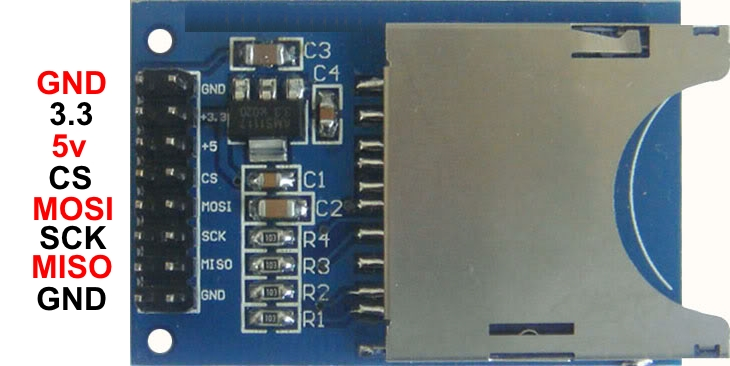
\includegraphics[scale=0.6]{figuras/cartaosdpinagem}
	\caption{Imagem ilustrativa do módulo de cartão de memória SD. Demonstra as funções de cada pino.}
	\label{cartaosdpinagem}
\end{figure}
%%\FloatBarrier

Sensor de Condutividade

A condutividade elétrica é a habilidade de um material permitir a passagem de corrente elétrica. A corrente elétrica flui na água através de íons. A quantidade de íons, o tipo dos íons e a temperatura do eletrólito influenciam na condutividade da água.
A condutividade da água também é um indicador de qualidade. A magnitude da condutividade propriamente dita não é importante, mas sim as variações abruptas que podem ocorrer durante um período de medição. A variação da condutividade na água significa que houve aumento significante de alguma substância. Um vazamento de esgoto, ou poluição por água residual agrícola irá aumentar a condutividade da água por possuir elementos como nitrato, fosfato e cloreto. Poluição causada por óleo ou qualquer matéria orgânica diminuirá a condutividade da água por serem elementos que não se dividem em íons.
Este sensor consiste em duas pontas de prova metálicas submersas numa solução aquosa. O princípio de medição deriva da lei de Ohm, em que a tensão aplicada nos terminais de um condutor é proporcional à corrente elétrica que o percorre. Para medir a condutividade da água é importante levar em consideração o efeito de polarização, eletrólise e a capacitância gerada oriunda das duas pontas metálicas em um meio dielétrico. Para evitar, ou diminuir, estes efeitos, deve ser utilizado um sinal de corrente alternada com frequência elevada. Por conseguinte, os íons não irão conseguir se depositar nas pontas metálicas e tampouco criar uma região polarizada. Assim, o sensor consistirá de três blocos principais.
\begin{itemize}
	\item Oscilador
	\item Amplificador
	\item Conversor A/D
\end{itemize}

O circuito oscilador Ponte de Wien é um oscilador simples capaz de gerar ondas sinusoidais por meio de um amplificador operacional com realimentação positiva.
O bloco amplificador será utilizado para obter valores significativos de tensão que possam ser, posteriormente convertidos em sinal digital para, em seguida, ser traduzido em informação útil e, por final, transmitido. Este sensor, por sua simplicidade, também será desenvolvido pela equipe.
Os desafios são os mesmos comparado ao sensor de turbidez. A dificuldade e riscos estarão presentes na confecção da ponta de prova e também na calibração do dispositivo.

Sensor de turbidez
 
Turbidez é a medição da quantidade de luz dispersada pela interação de luz incidente com matéria suspensa não dissolvida em uma amostra de água. A turbidez pode ser interpretada como a medida da transparência da água e geralmente indica a presença de sólidos suspensos como limo, argila, silicatos, algas, matéria orgânica ou inorgânica, e até mesmo a presença de microrganismos. Estes sólidos suspensos contribuem para a cultura de microrganismos patogênicos por fornece-los abrigo e alimento. Além disso, dificultam o tratamento da água para sistemas de distribuição, quando por exemplo, há grande quantidade de matéria orgânica, aumentando a demanda por cloro. Estes patogênicos, caso não tratados corretamente, podem causar problemas gastrointestinais oriundos de água de má qualidade. Para ecossistemas aquáticos, a turbidez confere um aspecto importante aos organismos fotossintetizantes aumentando ou diminuindo sua concentração em determinadas áreas e, assim, afetando, por exemplo, a cadeia alimentar local. A importância da monitoração da turbidez se estende da qualificação de água potável a sistemas aquáticos naturais.
Os métodos existentes para medir a transparência da água muitas vezes exigem interferência humana, tais como vela de Jackson e tubo de Secchi, que consistem em analisar a transparência da água via visualização. Estes métodos estão descartados por demandar interferência humana, baixa precisão para pequenos volumes de água, e por impossibilitar a medição de forma remota. Para cumprir com os requisitos do projeto, a medição deve ser feita remotamente, deve ser precisa e realizada em tempo real, necessitando uma abordagem mais moderna. Existem três possíveis abordagens para medir a turbidez da água, todas usando emissores e receptores de luz em que seus resultados dependem da quantidade de sólidos suspensos, tamanho das partículas, formato das partículas, reflexibilidade das partículas.
·         Nefelômetro: este método mede a dispersão de luz com um sensor a 90 em relação à fonte de luz. Este método mede diretamente a luz dispersa pelas partículas. O nefelômetro é mais extremamente sensível e utilizado em amostras com baixa turbidez.
·         Turbidimetro: O turbidímetro mede a diferença na intensidade, ou energia, da luz que chega ao receptor colocado em frente ao emissor de luz.
·         Existem um terceiro dispositivo que é a junção dos dois métodos citados acima, e possui a vantagem de obter leituras independentes da coloração do liquido analisado.
Como explicado anteriormente, o nefelômetro consiste de um sensor de luz orientado a 90 graus da fonte emissora de luz, como mostra a figura a seguir:



A proposta do grupo é confeccionar o sensor, utilizando um LED infravermelho ou um diodo laser como emissor e um fotodiodo como receptor. Confeccionar também todo o circuito para o tratamento do sinal, como um amplificador de transimpedância, para que seja obtido um sinal de tensão. Além disso, calibrar o sensor para obtenção de medições confiáveis e precisas. A confecção deste sensor é viável e irá reduzir os custos do projeto.
Os maiores riscos previstos para a implementação deste dispositivo é a fabricação da ponta de prova que entrará em contato com a água, o posicionamento correto do emissor e do receptor e, por fim, a calibragem.

Sensor de temperatura

O sensor de temperatura digital DS18B20 é capaz de medir em graus Celsius, com resolução de 9-bit a 12-bit (configurável) e possui uma função de alarme programável em memória não volátil para valores abaixo ou acima das temperaturas desejadas. A comunicação é feita por 1- fio, ou seja, precisa apenas de 1 pino do microcontrolador para transferir os dados. Pode operar entre -55ºC até +125ºC e com precisão de mais ou menos 0.5ºC se estiver operando dentro da faixa de -10ºC até +85ºC. Cada DS18B20 possui um número serial único de 64-bit, o que permite que vários DS18B20 funcionem no mesmo barramento 1- fio, permitindo conectar vários sensores em um microcontrolador.

É superior aos modelos DS1820 e DS18S20.

Características:

- Comunicação 1-fio, que necessita apenas de um pino do microcontrolador para fazer a linha de dados;
- Opera de 3V a 5.5V e pode ser alimentado pela linha de dados;
- Opera entre -55ºC até +125ºC, sendo a precisão de mais ou menos 0.5ºC se estiver operando dentro da faixa de -10ºC até +85ºC;
- resolução configurável pelo usuário de 9-bit à 12-bit;
- possui função de alarme programável;
- possui número de série único de 64-bit, o que permite ligar vários sensores no mesmo microcontrolador;

 \begin{figure} [!htp]
	\centering
	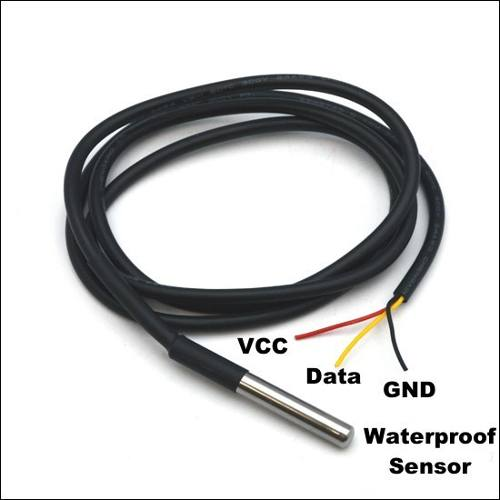
\includegraphics[scale=0.6]{figuras/sensortemp}
	\caption{Sensor para adquirir dados de temperatura.}
	\label{sensortemp}
\end{figure}
%%\FloatBarrier

Sensor de PH

\section{Subgrupo Estrutura}



